\documentclass[10pt, a4paper,english,spanish]{article}

% \usepackage{a4wide}
\parindent = 0 pt
\parskip = 11 pt
\usepackage[width=15.5cm, left=3cm, top=2.5cm, height= 24.5cm]{geometry}
%Margenes de la pagina.  otra opcion, usar \usepackage{a4wide}
%\usepackage[paper=a4paper, left=0.8cm, right=0.8cm, bottom=1.3cm, top=0.9cm]{geometry}
\usepackage{color}
\usepackage{amsmath}
\usepackage{amsfonts}
%este paquete permitcodebe incluir acentos.  Notar que espera un formato ANSI-blah de archivo.  Si en lugar de eso se tiene un utf8 (usual en los linux), entonces usar \usepackage[utf8]{inputenc}
\usepackage[utf8]{inputenc}
\usepackage{userStories}
\usepackage{tcolorbox}

%Este paquete es para que algunos titulos (como Tabla de Contenidos) esten en castellano
\usepackage[spanish]{babel}

%El siguiente paquete permite escribir la caratula facilmente
\usepackage{caratula}

\usepackage{framed}

\usepackage{graphicx}
\usepackage{float}

\usepackage{algorithm}
\usepackage{algorithmic}

%\usepackage{algpseudocode}

\newcommand{\real}{\mathbb{R}}
\newcommand{\nat}{\mathbb{N}}

\newcommand{\revJ}[1]{{\color{red} #1}}

%Datos para la caratula
\materia{Ingeniería de Software II}

\titulo{Reentrega del Trabajo Práctico 1}
\subtitulo{Planificación y Diseño Orientado a Objetos}

\integrante{Laporte, Matías}{686/09}{matiaslaporte@gmail.com}
\integrante{Salegas, Matías}{750/01}{matias.salegas@gmail.com}
\integrante{Vallejo, Nicolás}{500/10}{nico\_pr08@hotmail.com}
\integrante{Zanitti, Gastón}{058/10}{gzanitti@gmail.com}

\begin{document}

%esto construye la caractula
\maketitle 

\tableofcontents
  \newpage

\section{Introducción}
\indent \indent Esta primera etapa del trabajo consistió en la planificación, utilizando la metodología ágil Scrum, del desarrollo de un simulador de partidos de básquet de fantasía.

\subsection*{User Stories}
Por las características del sistema pedido, donde hay una simulación -que lleva una porción importante de cómputo y representa una etapa del desarrollo bastante \emph{pesada}-, quedaron pocas user stories en total, pues gran parte del sistema se concentra específicamente en ese punto. Esto fue algo que se habló con el tutor y estaba dentro de lo esperable.

Justamente por ser algo que llevaba tanto tiempo, se estuvo en la duda de si convenía o no dividir la \textbf{User Story} correspondiente a la simulación. Una solución propuesta fue especificar en las user stories que una simulación se componía de turnos, éstos de jugadas, y éstas de acciones de los jugadores. Una división de ese modo resultó exagerada, y además iría en contra del principio de independencia para las user stories de \textbf{Scrum}; dado que la simulación debería entrar completa en un único sprint, por lo tanto, se decidió dejarla como una única \textbf{User Story}.


\subsubsection*{Valuación User Stories}
Tanto para la sección de \emph{Business Value} como de \emph{Effort} de cada User Story se decidió realizar poker planning entre los 4 integrantes del grupo. Cuando había discrepancias, se esgrimían los argumentos por los que cada uno había puesto el puntaje correspondiente, de manera de intentar convencer a los otros y así converger los criterios.

\subsection*{Roles}
Otro punto donde hubo ciertas dudas acerca de si se estaba o no en uno de los muchísimos caminos correctos posibles, fue en cuanto a los roles. A primera vista, no parecería haber nadie más que participe del sistema más que el usuario final, a quien llamamos un \emph{participante}. 

Leyendo con un poco más de atención y por cómo se encontraban redactados algunos puntos específicos del enunciado, dejando algunas cosas abiertas con la posibilidad de que sufran modificaciones a futuro, nos pareció propicio considerar un rol de alguien que se encarga de ``mantener'' y administrar el sistema -que seguramente no sea el \emph{dueño}, aunque sí puede que esté dirigido por el mismo-. Ese sería el rol del \emph{administrador}.


\begin{itemize}
\item \textbf{Participante}: es quien se encarga de crear equipos, desafiar a otros participantes y participar de las simulaciones. El \textit{usuario final} del sistema.
\item \textbf{Administrador}: es aquel que actualiza los datos de los jugadores, define las jugadas de cada técnico y las configuraciones de la simulación, tales como la cantidad de turnos de cada una. Es un supervisor del sistema, quien lo regula, el que realiza las acciones para hacerlo más atractivo para los participantes, y más equilibrado.
\end{itemize}

  \newpage
\section{Plan de Proyecto}
\label{sec:planificacion}
\subsection{Iteraciones}
Las iteraciones tienen una duración aproximada de 3 semanas (15 días hábiles). Teniendo en cuenta que los recursos asignados son 4 arquitectos de software/programadores trabajando de modo part-time (6 horas), se estiman unas 360hrs. aproximadas por iteración.

Nuestra decisión sobre la conformación de las iteraciones -en cuanto a los casos de uso- se rigió por varios factores: 
\begin{itemize}
\item Se tuvieron en cuenta las necesidades extraídas del QAW con los stakeholders
\item Se trató de agrupar a los casos de uso por su temática, prefiriendo en caso de ser posible juntar dentro de una misma iteración los casos de uso que se relacionan con funcionalidades similares.
\item Otro factor que se tuvo en cuenta a la hora de definir el orden de las iteraciones, fueron los riesgos detectados y analizados en la sección de Análisis de Riesgos (\ref{sec:riesgos}).
\item También se consideró la prioridad de la funcionalidades referidas en los casos de uso, intentando en lo posible desarrollar antes las más importantes para el negocio.
\end{itemize}

La primera iteración quedó expresamente definida por el QAW y el análisis de riesgo, factores a los que se les dio mayor prioridad. 
Del análisis de riesgo, y dado el factor prioritario que tiene la disponibilidad del sistema, se extrajo que la parte más conflictiva ocurre a la hora de transmitir los desafíos (especialmente para los eventos globales), así como al mostrar correctamente las simulaciones.

El siguiente punto en cuanto a nivel de riesgo, fue lo concerniente a la seguridad, integridad y transparencia de la transmisión de los datos de pago y movimientos de dinero, y las transmisiones de datos usadas para definir los resultados de los partidos de la realidad y minuto a minuto de las simulaciones. Decidimos encarar esto en la segunda iteración del proyecto.

Otro foco de preocupación y de vital importancia para el proyecto, es su alcance y monetización. Por esa razón, se decidió trabajar en lo que respecta a las publicidades del sitio, simulaciones y transmisiones (y el uso de los datos de comportamiento de usuarios), además de la regionalización del sistema (con todas las reglas y restricciones que eso conlleva) en la tercer iteración.

El manejo administrativo de las cuentas de los usuarios, y el aspecto \emph{social} (chat, utilización de las opiniones vertidas en redes sociales, etc.), consideradas cuestiones de menor complejidad, se decidieron enfrentar en la cuarta iteración.

Decidimos dedicarnos en la quinta iteración a todo lo referido a los desafíos, su creación, configuración, definición de reglas y de los premios. En la sexta iteración, nos encargaremos de lo que concierne a los rankings de los jugadores globales, regionales, etc. Como los casos de uso de estas dos iteraciones tienen un menor riesgo y complejidad que los anteriores, consideramos que estas dos fases son de construcción, ya que se trabajará bastante en lo implementativo y poco en el análisis/diseño.



\subsubsection{I01 - Primera Iteración (Elaboración)}
\begin{itemize}
\item (CU19) Mostrando detalle minuto a minuto de la simulación
\item (CU2)  Obteniendo datos en tiempo real
\item (CU21) Mostrando simulación gráfica
\item (CU22) Observando la transmisión de un partido de liga
\item (CU20) Observando evento global/continental
%\item CU15) Mostrando desarrollo (log o streaming) de desafío} (sistema -> usuario)
\end{itemize}

\subsubsection{I02 - Segunda iteración (Elaboración)} 
\begin{itemize}
\item (CU9) Creando cuenta de usuario
\item (CU10) Actualizando datos de medios de pago
\item (CU34) Auditando movimientos de dinero
\item (CU33) Consultando estado de cuenta y movimientos de usuario
\item (CU35) Auditando simulaciones
\item (CU8) Apostando
%\item CU43) Logueando movimientos de dinero}: (depende de lo que diga Javi)
\end{itemize}


\subsubsection{I03 - Tercera Iteración (Elaboración)}
\begin{itemize}
\item (CU36) Definiendo restricciones por zona
\item (CU25) Definiendo regiones de la plataforma
\item (CU18) Definiendo reglas de simulación
\item (CU38) Configurando publicidad y ads en transmisiones
\item (CU16) Configurando publicidad en el sitio y simulaciones
\item (CU17) Acceder a datos de preferencia/comportamiento de usuarios
%\item (CU44) Mostrando publicidad en la simulación} - ¿es algo que se hace al generar la simulación,  puede ser luego?
%\item (CU37) Configurando publicidades en simulaciones y en el sitio}:  (representante de empresas (?))
%\item (CU39) Consultando datos de usuario}: (representantes de empresas(?))
\end{itemize}


\subsubsection{I04 - Cuarta Iteración (Elaboración)}
\begin{itemize}
\item (CU6) Participando del chat general
\item (CU7) Participando de chat privado
\item (CU12) Consultando cuenta de usuario
\item (CU41) Desactivando cuenta
\item (CU42) Reactivando cuenta
\item (CU23) Recolectando opiniones de redes sociales y chats
\item (CU24) Definiendo impacto de opiniones
%4- consultando datos de jugadores /técnicos /equipos (participante)
\end{itemize}

\subsubsection{I05 - Quinta Iteración (Construcción)}
\begin{itemize}
\item (CU1) Eligiendo liga para competir
\item (CU3) Definiendo reglas de desafío
\item (CU4) Creando desafío
\item (CU5) Aceptando desafío
\item (CU14) Consultando estado (cuenta regresiva, participantes, posiciones) del desafío
\item (CU13) Definiendo premios
\end{itemize}

\subsubsection{I06 - Sexta Iteración (Construcción)}
\begin{itemize}
\item (CU28) Consultando dashboard regional o global
\item (CU29) Consultando ranking de jugadores
\item (CU32) Reiniciando el ranking de jugadores
\item (CU26) Definiendo desafíos interzonales
\item (CU31) Configurando visibilidad de los desafíos
%6 -  definiendo reglas de puntajes (administrador)
\end{itemize}


\subsection{Primera iteración (I01) en detalle}
\label{subsec:primeraiteracion}
En esta sección se realiza un detalle de las tareas que se consideran necesarias realizar en la primer iteración, junto a las horas hombres esperadas. Dado que ya se realizó un reconocimiento, priorización, y estimación de tiempo de los casos de uso, además del análisis de riesgo, no serán tareas prioritarias ni de mucha intensidad en esta etapa, sino que se utilizarán para poder corregir detalles de las futuras iteraciones.

Algunas de las tareas (por ejemplo I01T01, I01T02, I01T03) que no se corresponden directamente con un caso de uso, tienen como objetivo la mitigación de los riesgos analizados (\ref{sec:riesgos}).

\begin{itemize}
\item \underline{I01T01} - Reunión semanal breve con stakeholders para asegurarse que los requerimientos estén actualizados: \textbf{10hs}.
  \begin{itemize}
    \item \underline{I01T01ST01} - Reunión la primer semana: 4hs.
    \item \underline{I01T01ST02} - Reunión la segunda semana: 3hs.
    \item \underline{I01T01ST03} - Reunión la tercer semana: 3hs.
  \end{itemize}
\hfill

\item \underline{I01T02} - Reunión cada 3 días hábiles del equipo para evitar problemas de comunicación como en el pasado: \textbf{10hs}.
  \begin{itemize}
    \item \underline{I01T02ST01} - Primera reunión: 2hs.
    \item \underline{I01T02ST02} - Segunda reunión: 2hs.
    \item \underline{I01T02ST03} - Tercer reunión: 2hs.
    \item \underline{I01T02ST04} - Cuarta reunión: 2hs.
    \item \underline{I01T02ST05} - Quinta reunión: 2hs.
  \end{itemize}
\hfill

\item \underline{I01T03} - Reunión semanal de consulta con experto en metodología UP: \textbf{8hs}.
  \begin{itemize}
    \item \underline{I01T03ST01} - Reunión la primer semana: 3hs.
    \item \underline{I01T03ST02} - Reunión la segunda semana: 2hs.
    \item \underline{I01T03ST03} - Reunión la tercer semana: 2hs.
  \end{itemize}
\hfill

\item \underline{I01T04} - Identificación y descripción de los atributos de calidad del sistema: \textbf{40hs}.
  \begin{itemize}
    \item \underline{I01T04ST01} - Cotejamiento de los atributos definidos por stakeholders en QAW y relación con los casos de uso definidos: 16hrs.
    \item \underline{I01T04ST02} - Descripción de escenarios de atributos de calidad: 20hs.
    \item \underline{I01T04ST03} - Verificación de la documentación escrita: 4hs.
  \end{itemize}
\hfill
  
\item \underline{I01T05} - Diseño de la arquitectura del sistema: \textbf{60hs}.
  \begin{itemize}
    \item \underline{I01T05ST01} - Analizar los escenarios descritos en I01T04 e identificar drivers de arquitectura: 8hs. 
    \item \underline{I01T05ST02} - Estudiar y elegir patrones arquitectónicos que satisfagan los drivers identificados: 12hs.
    \item \underline{I01T05ST03} - Verificar y refinar los casos de usos y los escenarios: 10hs.
    \item \underline{I01T05ST04} - Iterar: 30hs.
   \end{itemize}
\hfill

\item \underline{I01T06} - Realización de las tareas del (CU2)  Obteniendo datos en tiempo real: \textbf{40hs}.
  \begin{itemize}
    \item \underline{I01T06ST01} - Reunirse con empresas que provean datos en tiempo real de la evolución de los partidos y contratar alguna: 12hs.
    \item \underline{I01T06ST02} - Reunirse con la empresa contratada y obtener documentación técnica sobre la API que proveen: 2hs.
    \item \underline{I01T06ST03} - Investigar la API y analizar qué datos podemos usar como input en nuestro sistema: 6hs.
    \item \underline{I01T06ST04} - Adaptar nuestro sistema para que los desafíos en modo \emph{Liga de fantasía} utilicen los datos obtenidos a través de la api: 10hs.
    \item \underline{I01T06ST05} - Realizar algunos desafíos y verificar que los resultados de los puntajes se condigan con lo que ocurrió en los partidos reales: 6hs.
    \item \underline{I01T06ST06} - Corregir potenciales errores: 4hs.
  \end{itemize}
\hfill

\item \underline{I01T07} - Realización de las tareas del (CU19) Mostrando detalle minuto a minuto de la simulación: \textbf{40hs}.
  \begin{itemize}
    \item \underline{I01T07ST01} - Investigar el log del desarrollo anterior, cómo se genera y la calidad de la salida: 4hs.
    \item \underline{I01T07ST02} - Reunirse con las empresas desarrolladoras de los dos motoroes gráficos y averiguar qué tipo de entrada necesitan: 6hs.
    \item \underline{I01T07ST03} - Comparar el log actual con el que se necesita y definir qué es lo que falta agregar: 4hs.
    \item \underline{I01T07ST04} - Agregar el detalle necesario al log de salida para cumplir con lo requerido por las empresas: 10hs.
    \item \underline{I01T07ST05} - Ajustar la velocidad de salida del log para que no sea instantánea, sino minuto a minuto, y respete la nueva duración (similar a la de un partido real) de las simulaciones: 5hs.
    \item \underline{I01T07ST06} - Realizar algunas ejecuciones de prueba y obtener logs de salida de ejemplo: 4hs.
    \item \underline{I01T07ST07} - Corroborar con empresas proveedoras que el detalle del log obtenido sea el correcto: 2hs.    
    \item \underline{I01T07ST08} - Corregir potenciales errores: 5hs.
  \end{itemize}
\hfill

\item \underline{I01T08} - Realización de las tareas del (CU21) Mostrando simulación gráfica: \textbf{50hs}.
  \begin{itemize}
    \item \underline{I01T08ST01} - Reunirse con empresa de motor 3D y discutir sobre los requerimientos técnicos para la transmisión de video en dispositivos no soportados por el motor gráfico: 10hs.
    \item \underline{I01T08ST02} - Obtener varios logs minuto a minuto de prueba y utilizarlos como entrada para los distintos motores gráficos. Comparar que el resultado gráfico (según limitaciones de cada motor) de los partidos sea el mismo y no haya diferencias: 20hs.
    \item \underline{I01T08ST03} - Probar los motores en distintos dispositivos y obtener los requerimientos mínimos y recomendados de hardware para poder informar a los participantes: 15hs.
    \item \underline{I01T08ST04} - Escribir documentación sobre los distintos motores, obtener screenshots para poder publicar en el home del producto como ejemplo de jugabilidad: 5hs.
  \end{itemize}
\hfill


\item \underline{I01T09} - Realización de las tareas del (CU22) Observando la transmisión de un partido de liga: \textbf{65hs}.
  \begin{itemize}
    \item \underline{I01T09ST01} - Reunirse con la empresa dueña de los derechos de televisión y la empresa proveedora de infraestructura para definir sus requerimientos, necesidades, y llegar a acuerdos comunes en los puntos álgidos: 10hs.
    \item \underline{I01T09ST02} - Reunirse con la empresa proveedora de infraestructura de redes para definir la arquitectura de hardware a utilizar para el sistema: 8hs.
    \item \underline{I01T09ST03} - Implementar la solución de hardware convenida con la empresa proveedora de infraestructura de redes: 16hs.
    \item \underline{I01T09ST04} - Realizar pruebas internas de transmisión en vivo de eventos con diferentes cargas en los servidores y desde distintas regiones: 16hs.
    \item \underline{I01T09ST05} - Dar feedback a la empresa proveedora de infraestructura y ver, de ser necesario, cómo mejorar el rendimiento: 10hs.
    \item \underline{I01T09ST06} - Mostrarle a la empresa dueña de los derechos de televisión el funcionamiento del sistema y verificar que cumpla con sus requerimientos: 5hs.
  \end{itemize}
\hfill

\item \underline{I01T10} - Realización de las tareas del (CU20) Observando evento global/continental: \textbf{hs}.
  \begin{itemize}
    \item \underline{I01T10ST01} - : XXhs.
    \item \underline{I01T10ST02} - : XXhs.
    \item \underline{I01T10ST03} - : XXhs.
    \item \underline{I01T10ST04} - : XXhs.
  \end{itemize}
\hfill

La suma de las tareas para la primer iteración da ???hs. Habiendo calculado una iteración ideal de 360hs. nos da cierto margen como para poder afrontar tareas urgentes o no previstas.

\subsection{Diagrama de Gantt}
  
\end{itemize}

  \newpage
\section{Diseño}
A continuación se presentan y explican algunas de las desiciones de diseño elegidas durante el desarrollo del trabajo practico.
Se decidió dividir la presentación en subsecciones para facilitar la comprensión de la misma, haciendo especial enfasis en aquellas que sentiamos eran de importancia para la comprensión del mismo.

Vale mencionar que si bien es cierto que se genero una idea general en el grupo antes de comenzar a reflejar las decisiones tomadas en codigo, el diseño en profundidad se termino de desarrollar y afinar en paralelo, mientras surgian cuestiones mismas relacionadas al propio desarrollo que no habian sido tenidas en cuenta en papel. 

\subsection{Acciones}
Todas las jugadas que pueden desarrollarse durante la simulacion de un partido, se divide claramente en dos grupos. Aquellas que realiza el equipo que esta atacando, y aquellas que realiza aquel que esta defendiendo. En base a esta idea, planteamos nuestro diseño clasificando a todas las acciones que pueden realizarse dentro de una jugada, en alguno de estos dos grupos (Ofensivas y Defensivas) y sub clasificando luego, de acuerdo al tipo de accion.
Este diseño, ademas de presentar de forma simple la realidad, nos permite extender el modelo con nuevas acciones tanto ofensivas como defensivas, de manera relativamente sencilla. Bastaria simplemente con declarar una nueva clase de herede de el tipo de clasificacion correspondiente de la accion. Por supuesto, la accion conoce al jugador que la esta ejecutando para poder mantener la informacion de la simulación de forma consistente.
\begin{center}
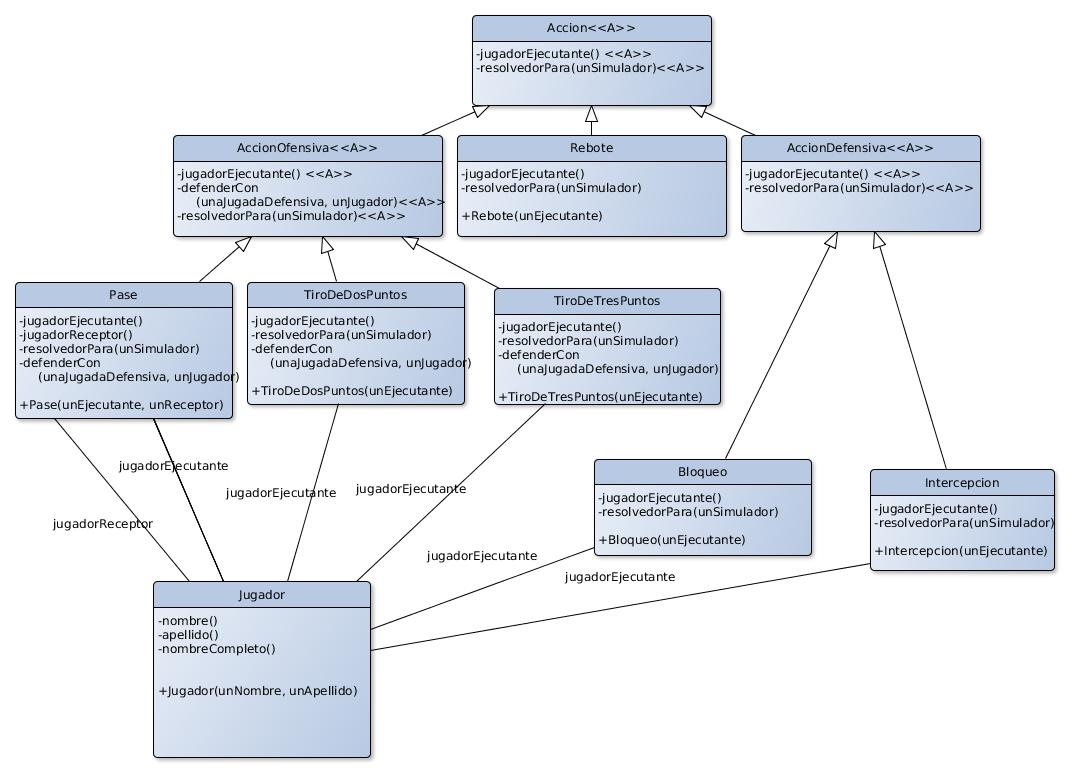
\includegraphics[scale=0.35]{diseno/acciones.jpg}
\end{center}

Veamos entonces como es que estas acciones se elijen y se ejecutan:
\begin{center}
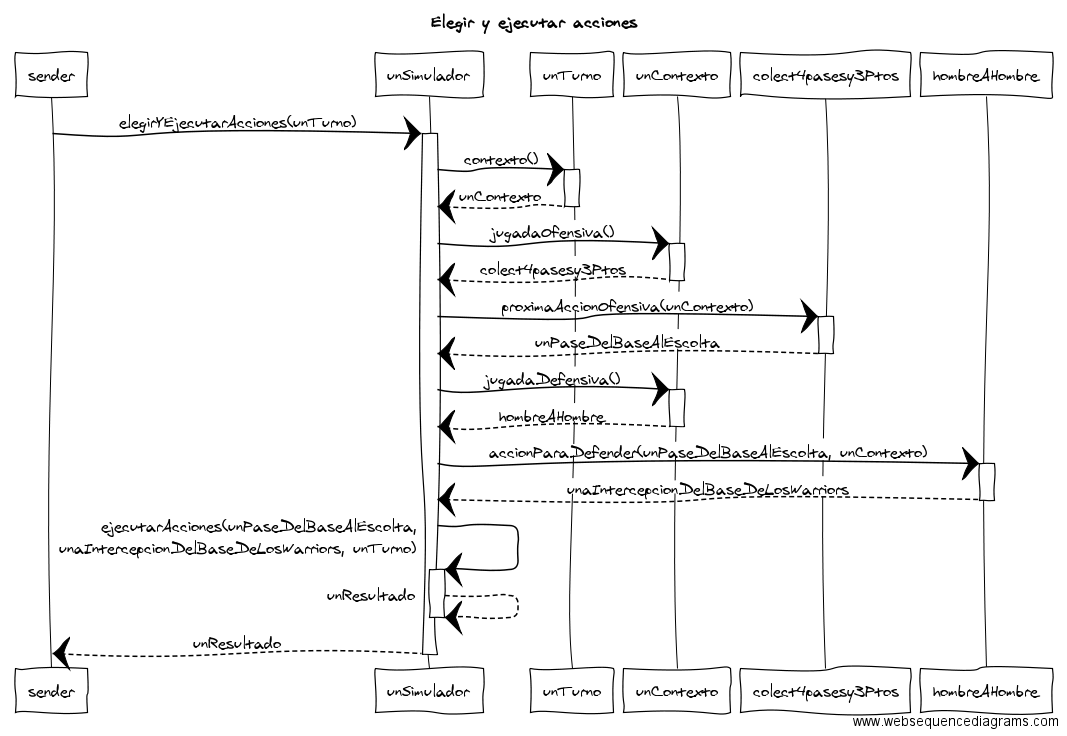
\includegraphics[scale=0.35]{diseno/Elegir_y_ejecutar_acciones.png}
\end{center}
Queda entonces claro como es que el simulador se encarga de tomar la jugada que se esta realizando del contexto y solicitarle las acciones correspondientes a cada una de estas para, luego de recibidas, proceder a ejecutarlas.

\subsection{Jugadas y acciones}
A continuación, presentamos entonces, como es que cada una de las acciones mencionadas en el apartado anterior, se integra con las jugadas defensivas/ofensivas, que componen los libros de los tecnicos.
\begin{center}
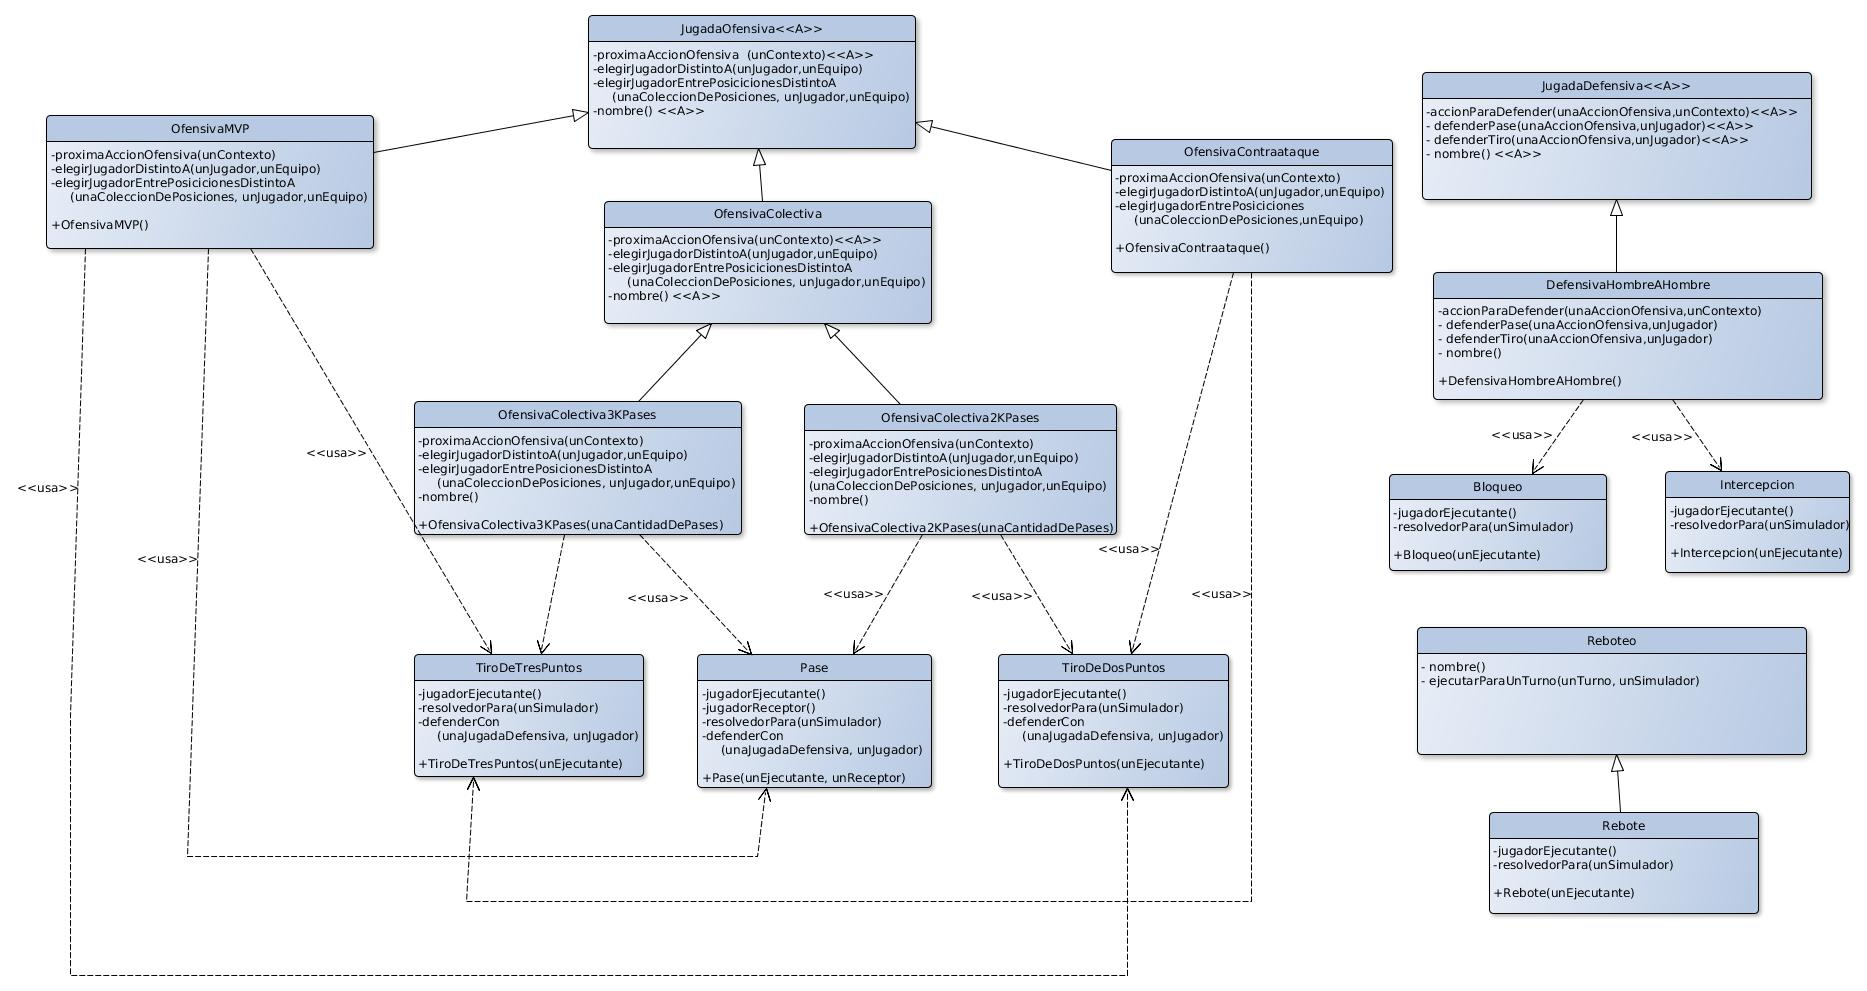
\includegraphics[scale=0.4, angle=90]{diseno/jugadasYAcciones.jpg}
\end{center}

En el siguiente diagrama de secuencia, podremos ver ademas, como estas distintas entidades encargadas de modelar las acciones de una jugada se relacionan con sus propios resolvedores. Estas ultimas son las entidades donde se calculan las distintas posibilidades de exito y fracaso para todas las interacciones entre dos jugadores. El hecho de que estos calculos no sean parte de las acciones en si, nos permite modificar los valores de las ecuaciones encargadas de calcular los resultados de cada accion de forma aislada y sin afectar al resto del modelo.

\begin{center}
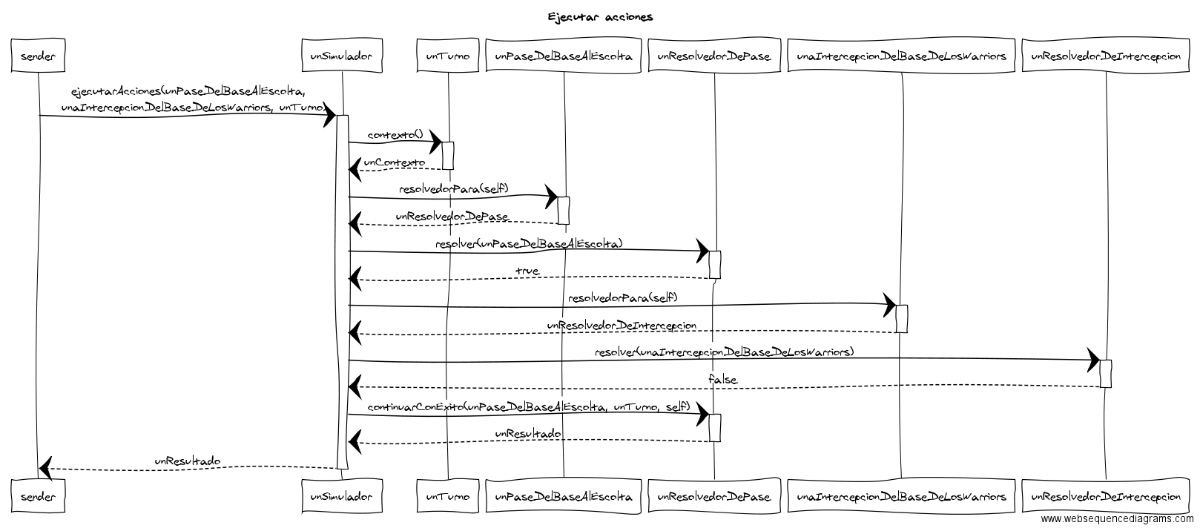
\includegraphics[scale=0.4, angle=90]{diseno/Ejecutar_acciones.png}
\end{center}


\subsection{Apuestas}
Decidimos que la mejor forma de clasificar las apuestas era mediante una jerarquizacion, para poder representar de forma clara que existen aquellas en las que se pone en juego un numero X de fichas, pero tambien aquellas nulas en las que no hay cap apostado. Esta clasificación, si bien es posible que agregue mas complejidad al diseño que suponiendo que las apuestas nulas son aquellas con cantidad de fichas igual a cero, nos ahorra de tener que manejar un unico tipo de apuesta y preguntar por la cantidad de fichas apostados todo el tiempo, permitiendo alijerar el manejo de las apuestas.
\begin{center}
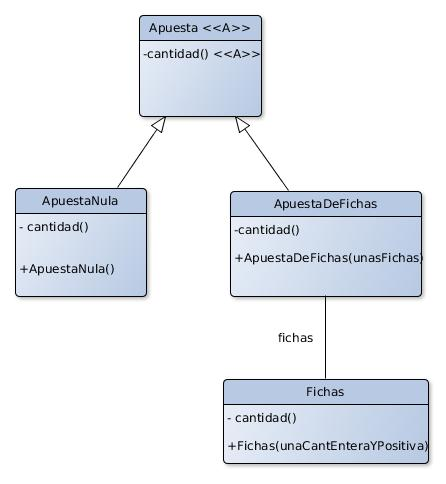
\includegraphics[scale=0.4]{diseno/apuestas.jpg}
\end{center}

\subsection{Equipo, jugadores y tecnico}
Para modelar al equipo, decidimos que exista una clase abstracta posición donde se hereden cada una de las posibles posiciones que puede adoptar un jugador. Nos parecio que es la forma mas correcta de representar la realidad, y si bien es cierto que en el tiempo las posibles posiciones no vayan a variar, nos permite diferenciar a cada jugador de manera sencilla a la hora de saber su interaccion dentro de una jugada. El tecnico, a su vez, cuenta con un libro de jugadas que puede usar tanto ofensivas como defensivas. Una forma simple de representar y distinguir ambas formas de juego.
\begin{center}
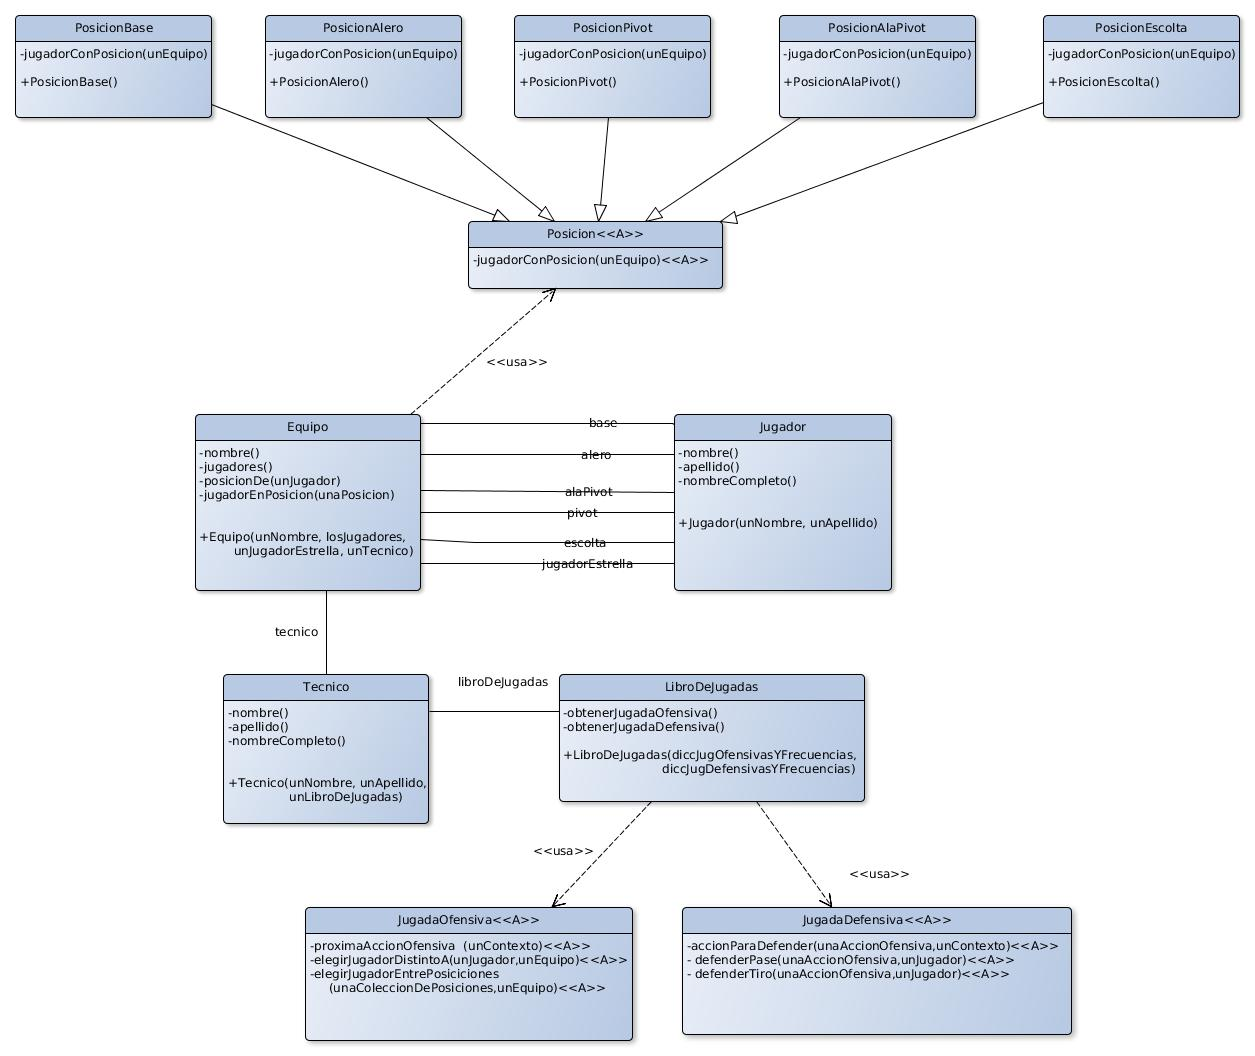
\includegraphics[scale=0.30]{diseno/equipo.jpg} 
\end{center}

A continuación veremos como se integran el tecnico con su libro de jugadas para elegir una jugada (en este caso, una ofensiva) con la simulación. Notese que, dado que las jugadas se eligen en base a la frecuencia de las mismas, se necesito de un generador de numeros aleatorios para simular el comportamiento de aleatoriedad en la eleccion de las mismas.
\begin{center}
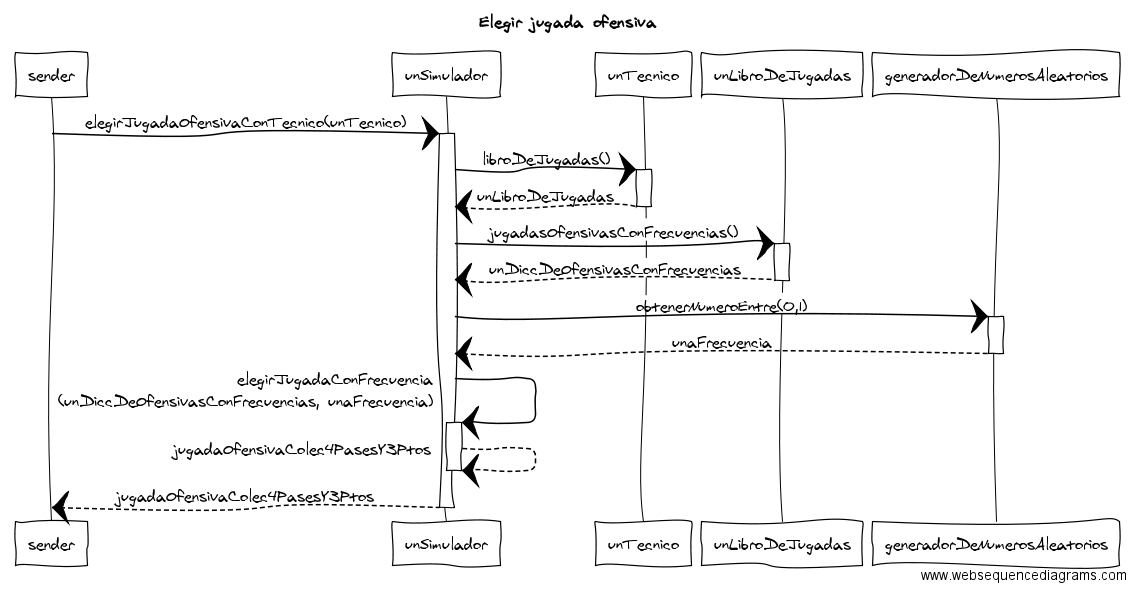
\includegraphics[scale=0.30]{diseno/Elegir_jugada_ofensiva.png} 
\end{center}

\subsection{Gestor de Equipos}
El gesto de equipos es aquel encargado de dar de alta y realizar cada una de las validaciones necesarias para confirmar la creacion de un equipo. Es por eso que se necesita de un gestor de Cap y una entidad que represente una lista de cada uno de los posibles jugadores. Esta elección nos permite disminuir la cohesión del modelo, permitiendo asi que futuras validaciones o modificaciones a las ya existentes, se agreguen de forma simple y sin agregar complejidad.
\begin{center}
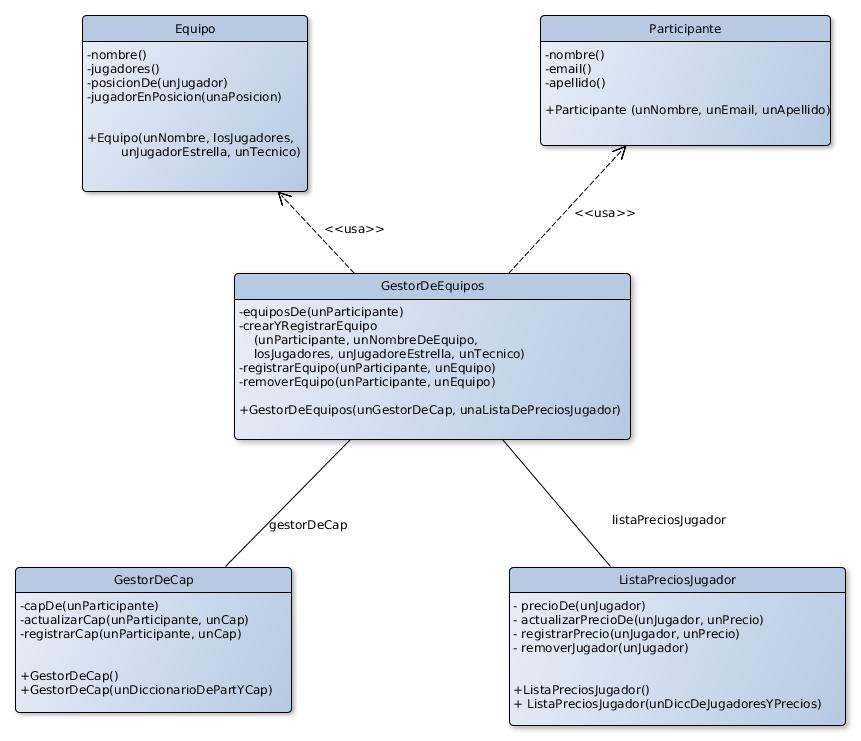
\includegraphics[scale=0.4]{diseno/gestorDeEquipos.jpg}
\end{center}

\subsection{Gestor de Cap y Fichas}
Estas dos entidades usan la misma logica y, conociendo al participante y la entidad a gestionar, permiten registrar y actualizar el cap y la cantidad de fichas de los participantes
\begin{center}
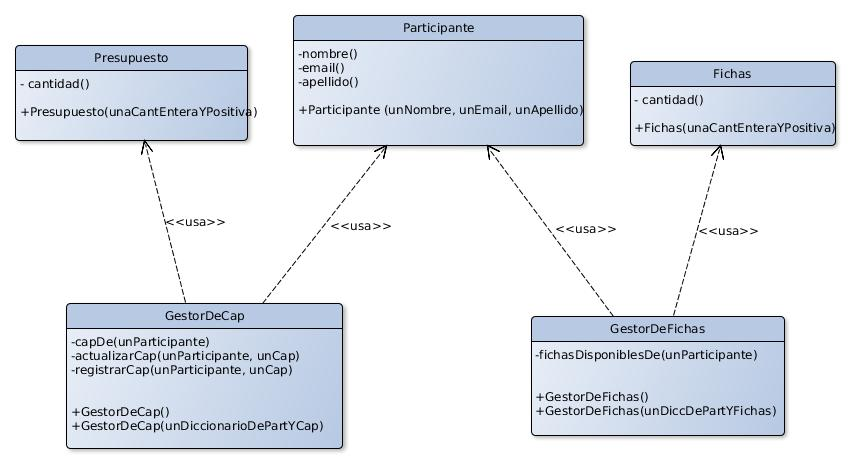
\includegraphics[scale=0.4]{diseno/gestorDeCapYFichas.jpg} 
\end{center}

\subsection{Registro de estadisticas}
Por ultimo, decidimos contar con una entidad encargada de llevar un registro de las estadisticas de cada uno de los jugadores porque no tenia sentido que un jugador sepa responder sus estadisticas. Esto nos permitia modelar la realidad de forma mas fehaciente, dejando abierta la posibilidad de cambios en las estadisticas de forma limpia para el futuro.
\begin{center}
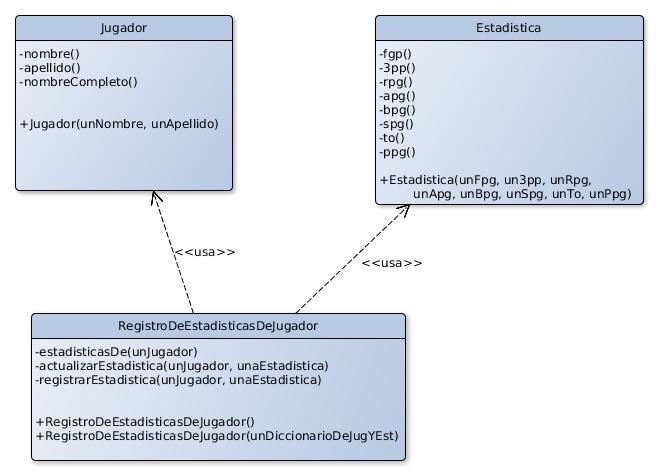
\includegraphics[scale=0.4]{diseno/registroDeEstadisticas.jpg}
\end{center}

\subsection{Partido}
Analicemos ahora el diagrama de clases de las entidades que componen un partido. Podemos ver, en un planteo un poco mas general, como se realiza tambien el loggeo de las distintas acciones que realizan los jugadores y como se integra la entidad resultados para poder dar cuenta de como finalizan las distintas acciones que mencionamos con anterioridad.
\begin{center}
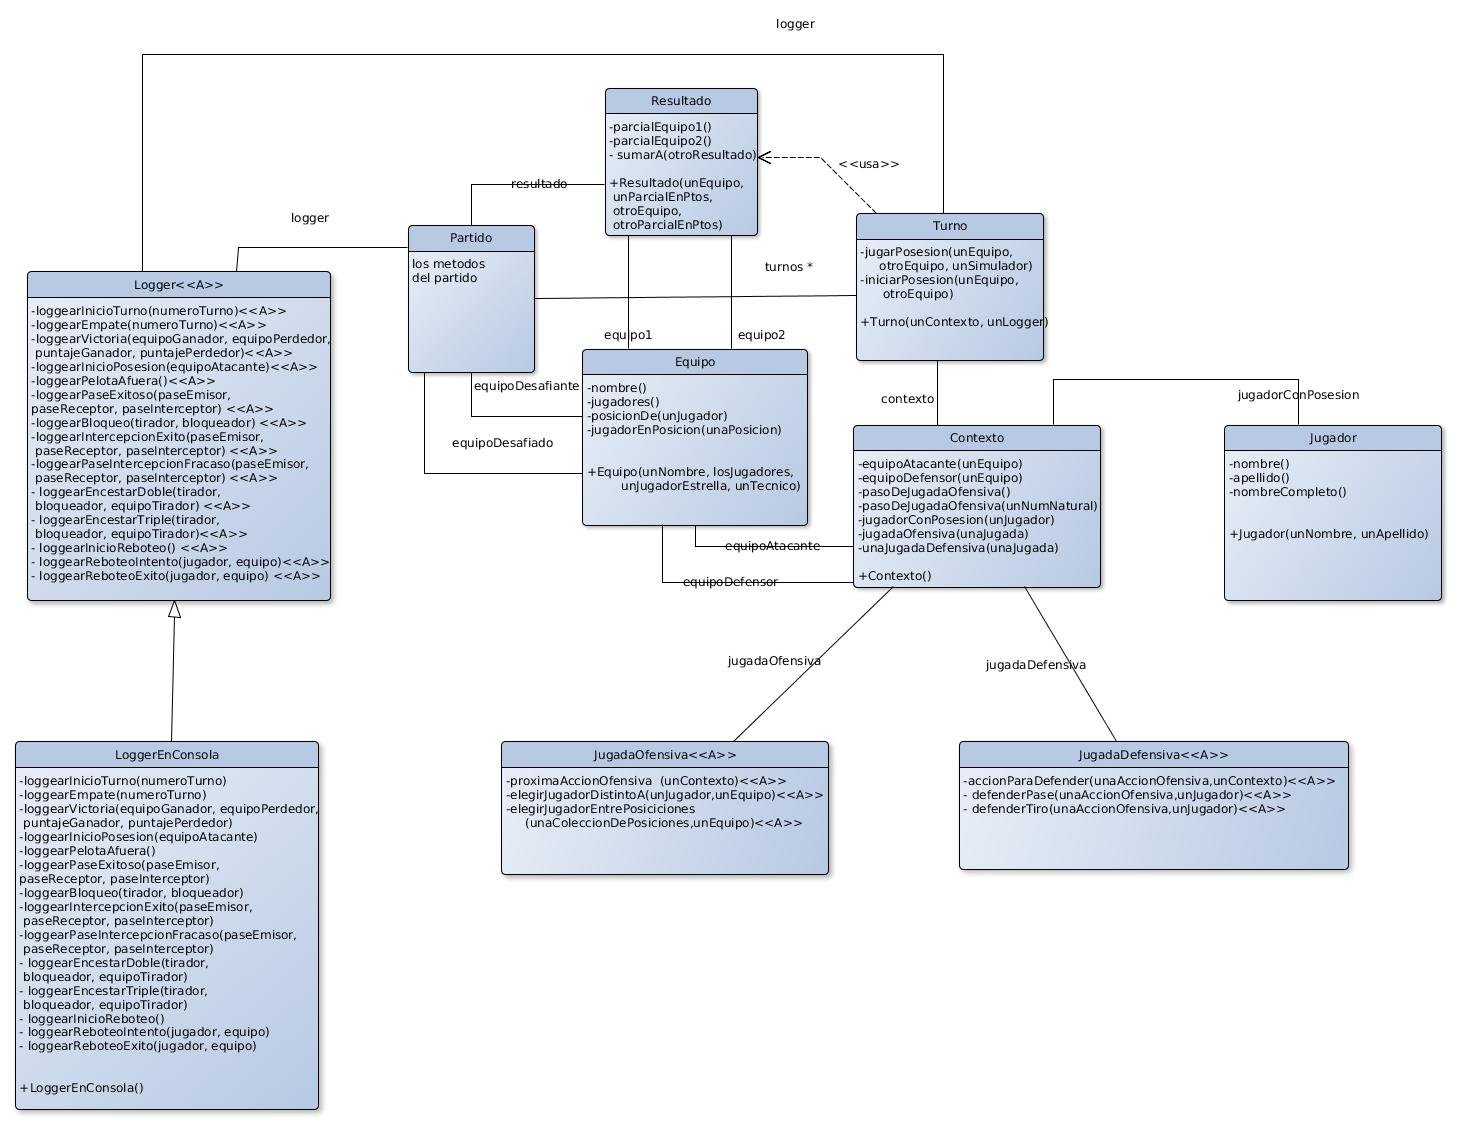
\includegraphics[scale=0.4, angle=90]{diseno/partido.jpg}
\end{center}


  \newpage
 \section{Organización de la Simulación}
La implementación de la demo de la simulación se organiza de la siguiente manera:
\begin{itemize}
 \item Un archivo main.py donde se cargan los datos de prueba y se inicia una simulación.
 \item Cuatro carpetas de aquellas clases que tienen alguna jerarquización (acciones, jugadas, resolvedores y posiciones), junto a sus clases herederas.
 \item El resto de las clases necesarias para correr una simulación.
\end{itemize}

Para correr una simulación, deberá ejecutarse el comando $python$ $main.py$ en una consola. Es posible ingresar previamente al archivo para modificar algunas estadísticas (dadas de alta de forma manual), el nombre de los equipos o de los jugadores, etc. y personalizar la salida por consola.

Además, se pueden modificar las ecuaciones utilizadas para calcular el éxito o fracaso de una acción, ingresando en la carpeta resolvedores y alterando los cálculos planteados en la función esExitoso() de cada uno de las clases correspondientes. 

  \newpage
\section{Sprint Retrospective}
El estado del TP entregado no es lo esperado ni lo solicitado, por lo que se torna difícil realizar conclusiones de cierre sobre algo que no cumple con esa condición, estar terminado. 

No se pudieron apreciar por completo las bondades ni dificultades de la metodología scrum porque decir que se siguió a rajatabla (dentro de la flexibilidad que ofrece) la metodología es una mentira. La dinámica del grupo no fue la esperada, con algunos desencuentros entre los integrantes, lo que dificultó considerablemente la tarea de llevar a cabo un desarrollo exitoso.

Algunos comentarios concernientes a la metodología que se podrían hacer son los siguientes:
\begin{itemize}
 \item Se sobreestimó la cantidad de horas que podría dedicarle cada integrante al grupo; si bien creimos que pusimos un número bastante conservador, ni siquiera se llegó a cumplir esa dedicación para el Trabajo Práctico. 
 \item Se subestimó la cantidad de horas para algunas tareas. No hay tareas que puedan llevar 0.5hrs, y muy pocas tareas que puedan llevar 1 hora. 
 \item Entre los dos items anteriores está claro cuán alejada estuvo finalmente la estimación de la realidad, y además, que en ambos puntos nos equivocamos en direcciones opuestas, aumentando aún más la famosa brecha.
 \item En base a lo vivido en el sprint, Scrum pareciera tener más sentido para un grupo reducido de personas que está cotidianamente en el mismo lugar, dedicándole una cantidad de horas similar a las tareas, y con una comunicación fluida y constante. La flexibilidad es una ventaja cuando se es dinámico y se tiene una adaptabilidad rápida a las distintas situaciones y problemáticas que van surgiendo a lo largo de la desarrollo. De ser esta conjetura cierta, el grupo no respetó bien ninguno de los puntos, y la falta de dinamismo e ida y vuelta ocasionó que no se pudieran tomar las decisiones necesarias en el momento indicado, retrasando todo.
 \item Es bastante difícil entrar en contacto con una metodología completamente desconocida para los integrantes en apenas unas semanas, y en el marco de una materia, donde además hay otras responsabilidades (relacionadas con la materia, con la Facultad, y las peores de todas, las ajenas a todo ello).
\end{itemize}



  \newpage
\begin{thebibliography}{9}

\bibitem{Gamma}
  Erich Gamma, Richard Helm, Ralph Johnson, John Vlissides.
  \emph{Design Patterns – Elements of Reusable Object-Oriented Software}.  
  Addison Wesley, 1995.

\bibitem{DoubleDispatch}
    Hebel, K., Johnson, R.. 
    \emph{Arithmetic and double dispatching in Smalltalk-80}.
    University of Illinois at Urbana-Champaign.

\bibitem{Teoricas}
    Santiago Ceria, Hernán Wilkinson, 
    \emph{Clases teóricas de Ingeniería de Software 2}.
    FCEN-UBA,
    2016.

\end{thebibliography}
  \newpage

\end{document}
